%        File: ans2012.tex
%     Created: Wednesday, January 25, 2012

\documentclass{anstrans}
%% To use the glossaries acronym package, you'll need to define any acronyms you intend to 
%% use. You can define acronyms with \newacronym{label}[acronym]{written out form}
%% To refer to them in the text use \gls{label}
\usepackage[acronym,toc]{glossaries}
\include{acros}
\makeglossaries


%%%%%%%%%%%%%%%%%%%%%%%%%%%%%%%%%%%
\title{Numerical Calibration of an Analytical Generic Nuclear Repository Heat 
Transfer Model}
\author{Kathryn D.~Huff$^1$, Theodore H.~Bauer$^2$}

%% uncomment these next five only if using anstrans
\institute{$^1$Nuclear Engineering \& Engineering Physics Dept., University of 
Wisconsin, Madison, WI, 53706\\
$^2$Nuclear Engineering Division, Argonne National Laboratory, Argonne, IL, 
60439}
\email{$^1$khuff@cae.wisc.edu \& $^2$thbauer@anl.gov}
\usepackage{graphicx}
\usepackage{booktabs} % nice rules for tables
\usepackage{microtype} % if using PDF
\usepackage{bigints}
\newcommand{\units}[1] {\:\text{#1}}%
\newcommand{\SN}{S$_N$}%{S$_\text{N}$}%{$S_N$}%
\DeclareMathOperator{\erf}{erf}


\date{January 27, 2012}
%%%%%%%%%%%%%%%%%%%%%%%%%%%%%%%%%%%
\begin{document}
%%%%%%%%%%%%%%%%%%%%%%%%%%%%%%%%%%%%%%%%%%%%%%%%%%%%%%%%%%%%%%%%%%%%%%%%%%%%%%%%
\section{Introduction}

This work describes a benchmarking effort between two generic geology nuclear 
repository heat transfer models and proposes an auxillary thermal resistance 
component to improve their agreement. The auxillary thermal resistance component 
improves the accuracy of the rapid analytic model by calibration against
the numeric model. 

The analytic model to be calibrated, created by \gls{LLNL}, calulates the 
superposition of line and point source solutions representing a generic geology 
nuclear repository. The auxillary thermal resistance calibration component 
suggested in this work improves the analytical model's estimation of the peak 
repository temperature as well as the timing of the peak temperature. The 
calibration was undertaken as part of a benchmarking effort against a 
geometrically detailed generic thermal nuclear repository thermal model 
developed at \gls{ANL} and based on the \gls{SINDAG} software\cite{SINDAG}.

%% RESULTS HERE %%

%%%%%%%%%%%%%%%%%%%%%%%%%%%%%%%%%%%%%%%%%%%%%%%%%%%%%%%%%%%%%%%%%%%%%%%%%%%%%%%%

%% The LLNL model

\section{Analytical LLNL MathCAD Model}

This model, created at \gls{LLNL} for the \gls{UFD} campaign seeks to inform 
heat limited waste capacity calculations for each lithology, for many waste 
package loading densities, and for many fuel cycle options. It employs an 
analytical model from Carslaw and Jaeger and is implemented in MathCAD. 
\cite{carslaw} The integral solver in the MathCAD toolset is the primary 
calculation engine for the LLNL thermal model, which relies on superposition of 
integral solutions.  

\subsection{Geometry}

\begin{figure}[h!]
  \begin{center}
    \includegraphics[width=0.5\textwidth]{llnlConcept.eps}
  \end{center}
  \caption{The central package is represented by a finite line source, adjacent 
  packages in the central drift are represented as points, and adjacent disposal 
  tunnes are represented as infinite lines.
  \cite{sutton_investigations_2011}.}
  \label{fig:llnl}
\end{figure}

\subsection{Calculation Method}

The model consists of two conceptual regions, a external and internal to the 
disposal tunnel wall.  The first `external' region is the host rock, and the second 
`interior' region is the tunnel region representing the waste form, package, and 
buffer. These are conceptualized to be a single `internal' calculation unit.  
Since the thermal mass of the \gls{EBS} is small in comparison to the thermal 
mass of the host rock, it may be treated as quasi-steady state. Thus, the 
transient state of the transient temperature at the host wall can be found with 
a MathCAD convolution of the sources outside the tunnel wall with the the 
superposition of integral solutions within the tunnel wall. 

The geometric layout of the analytical \gls{LLNL} model in Figure \ref{fig:llnl} shows  
that the central package is represented by the finite line solution
\begin{align}
  T_{line}(t,x,y,z) &= \frac{1}{8\pi K_{th}} 
  \bigintsss_0^t\!\frac{q_L(t')}{t-t'}e^{ \frac{-\left(x^2 + z^2\right)}{4\alpha 
  (t-t')} }\nonumber\\ 
  &\cdot\left[ 
  \erf{\left[ \frac{1}{2} \frac{\left( y + \frac{L}{2} 
  \right)}{\sqrt{\alpha(t-t')}}  \right]} 
  - \erf{\left[ \frac{1}{2} \frac{\left( y - \frac{L}{2} 
  \right)}{\sqrt{\alpha(t-t')}}  \right]} 
  \right]\,\mathrm{dt'},
  \label{line}
  \intertext{adjacent packages within the central tunnel are represented by the point source solution }
  T_{point}(t,r) &= \frac{1}{8K_{th}\sqrt{\alpha}\pi^{\frac{3}{2}}}\bigintsss_0^{-t}\!\frac{q(t')}{(t-t')^{\frac{3}{2}}}e^{\frac{-r^2}{4\alpha(t-t')}}\,\mathrm{dt'},
  \label{point}
  \intertext{and adjacent disposal tunnels are represented by infinite line source solutions}
  T_{\infty line}(t,x,z) &= \frac{1}{4\pi K_{th}} 
  \bigintsss_0^t\!\frac{q_L(t')}{t-t'}e^{ \frac{-\left(x^2 + z^2\right)}{4\alpha 
  (t-t')} }
  \intertext{in infinite homogeneous media, where}
  \label{infline}
  K_{th} &= ~~\mbox{thermal conductivity} [W/m\cdot K]\nonumber\\
  \alpha &= ~~\mbox{thermal diffusivity } [m^2/s]\nonumber\\
  q(t) &= ~~\mbox{point heat source} [W]\nonumber\\
  \intertext{and}
  q_L(t) &= ~~\mbox{linear heat source} [W/m]\nonumber
\end{align}
Superimposed point and line source solutions allow for a notion of the 
repository layout to be modeled in the host rock. Transient effects are achieved 
by the convolution of the external region solution with the internal region 
solution at the calculation radius. The process is then iterated with a one year
resolution in order to arrive at a temperature evolution over the lifetime of the repository. 
%% The ANL model

\section{Numerical ANL Model}

A similar model was created by the UFD team at \gls{ANL} using the \gls{SINDAG} 
heat transport framework employs a detailed numerical model model. It was created to 
model two distinct geometric arrangements, a single drift model and an infinite drift model.  
For a given waste stream, tunnel radius, and geologic parameters (i.e.  thermal 
conductivity, density, and specific heat capacity), the model is able to arrive  
at the temperature at the tunnel wall and adjacent. It can be run with an 
optimization loop to arrive at a minimal drift spacing for a given waste stream 
in agreement with user input thermal limits, but in this validation effort it was run 
deterministically from fiducial benchmark parameters. 

\subsection{Calculation Method}

The \gls{SINDAG} calculation engine uses a lumped parameter numerical model.

Originally created for optimal waste loading analysis of the \gls{YMR}, the 
model is geometrically adjustable in two dimensions,  as is demonstrated in 
Figure \ref{fig:sindageom}. The tunnel size is a fixed parameter in the model, 
but the optimal drift spacing for a particular waste stream and package loading 
is solved for with an optimization loop within this model.

\begin{figure}[htbp!]
  \begin{center}
    \includegraphics[width=0.5\textwidth]{./sindageom.eps}
  \end{center}
  \caption{The geometry of the thermal model can be adjusted in two dimensions, 
  altering the tunnel spacing and the vertical distance from the aquifer.}
  \label{fig:sindageom}
\end{figure}

The \gls{SINDAG} lumped capacitance solver solves a thermal circuit, for which 
conducting nodes may be of four types corresponding to the four modes of heat 
transfer. Nodes are connected by conduction, convection, radiation, and mass 
flow heat transfer links. As discussed in section \ref{sec:lumpedparam}, these 
are represented by

\begin{align}
  R_{cond} &= \frac{L}{k A}\\
  R_{conv} &= \frac{1}{h A}\\
  R_{mf}  &= \frac{1}{\dot{m}c_p}\\
  R_{rad}  &= \frac{1}{\sigma F_{ij}A\left[ T_i + T_A + T_j + T_A 
  \right]\left[(T_i+T_A)^2+(T_j+T_A)^2\right]}
  \intertext{where}
  k&= ~~\mbox{thermal conductivity}[W\cdot m^{-1}\cdot K^{-1}]\nonumber\\
  A&= ~~\mbox{area} [m^2]\nonumber\\
  c_p&=~~\mbox{specific heat capacity} [J\cdot K^{-1}]\nonumber  \\
  h&= ~~\mbox{heat transfer coefficient}[W\cdot m^{-1} \cdot K^{-1}\nonumber \\
  \dot{m}&= ~~\mbox{mass transfer rate}[kg\cdot s^{-1}]\nonumber \\
  T_i&= ~~\mbox{lump temperature} [^{\circ}C] \nonumber\\
  T_A&= ~~\mbox{absolute temperature} [^{\circ}C] \nonumber\\
  F_{ij}&= ~~\mbox{radiation interchange factor} [-] .\nonumber
\end{align}

With these representations of thermal resistance, a lumped parameter model will 
require an analysis that determines the appropriate length scale for the lumped 
parameter approximation.

Given one or more heat constraints, the \gls{ANL}  model  optimizes spatial 
waste loading in order to meet those constraints with maximal waste loading. For 
example, given a constraint at the edge of the waste package, the model utilizes 
the \gls{SINDAG} lumped capacitance solver to determine the two dimensional heat 
evolution of the repository as a result of a given waste package composition for 
various drift spacings and arrives at an ideal drift spacing by iteration.

\subsection{Geometry}

Two \gls{SINDAG} model geometries have been used in this benchmark.  

\subsubsection{Single Drift}

In the single drift geometry, there is a distant fixed boundary condition and 
one waste tunnel is modeled with a continuous, cylindrical heat source of 
infinite length. The linear heat source in $[\frac{W}{m}]$ is modeled as if it 
is spread radially onto the surface of the drift tunnel. 

\subsubsection{Multiple Drift}

In the multiple drift geometry, there is a reflective boundary condition at the 
mid-drift point. This results in a model that has an infinite number of infinite 
line source drifts.

\subsection{Detail}

The numerical detail available to the \gls{ANL} \gls{SINDAG} model has been 
shown historically to be consistent and applicable to repository regulation 
applications.


% Geometries

% Equations

%% Benchmarking


% Cases run : single drift in salt and clay, inf drift clay, finite drift clay

% Summary of Discrepancies

% Theory about source of Discrepancies


%% Calibration

% Auxillary Resistance Model

% Notion

It is assumed that \gls{EBS} compenents within the disposal tunnel are only a 
small volume fraction of the rock and that the temperature field in the \gls{EBS} 
respond to changes in the waste package decay heat more rapidly than the field 
in the surrounding host rock.

% Equation
\begin{align}
  \Delta T &= \frac{q}{L} \frac{1}{K_{th}}\frac{1}{D_d}\\
  \intertext{where}
  K_{th} &= \mbox{Thermal Conductivity}
  \label{deltat}
\end{align}


% Image

% Procedure for Fitting to ANL numerical model




Solution Method
The transient host rock thermal model is solved directly on the basis of host 
rock material properties, boundary conditions, and the heat generated by any 
enclosed storage units. Generated heat is included through simple “point” or 
“line” sources within host rock nodes.  Temperature fields within each storage 
unit are determined by a steady-state solution of the storage unit model 
assuming its known heat generation rate and using the temperature in the 
surrounding host rock (as determined from the host rock model) as a nearby 
boundary condition. 

Calibration occured for geologies of interest.  


%%%%%%%%%%%%%%%%%%%%%%%%%%%%%%%%%%%%%%%%%%%%%%%%%%%%%%%%%%%%%%%%%%%%%%%%%%%%%%%%


\section{Description of the Actual Work}

\subsection{Benchmarking}

A benchmarking effort between the analytical \gls{LLNL} model and the 
\gls{SINDAG} \gls{ANL} model revealed a discrepancy between them. The time of 
peak heat arrived sooner and the value of the peak temperature was lower in the 
homogeneous medium \gls{LLNL} model than in the \gls{SINDAG} model. 

% Cases Run

% Summary

% Theory


\subsection{Calibration}

\section{Results and Analysis}

%% Results

% Table

\begin{figure}[h!]
  \centering
    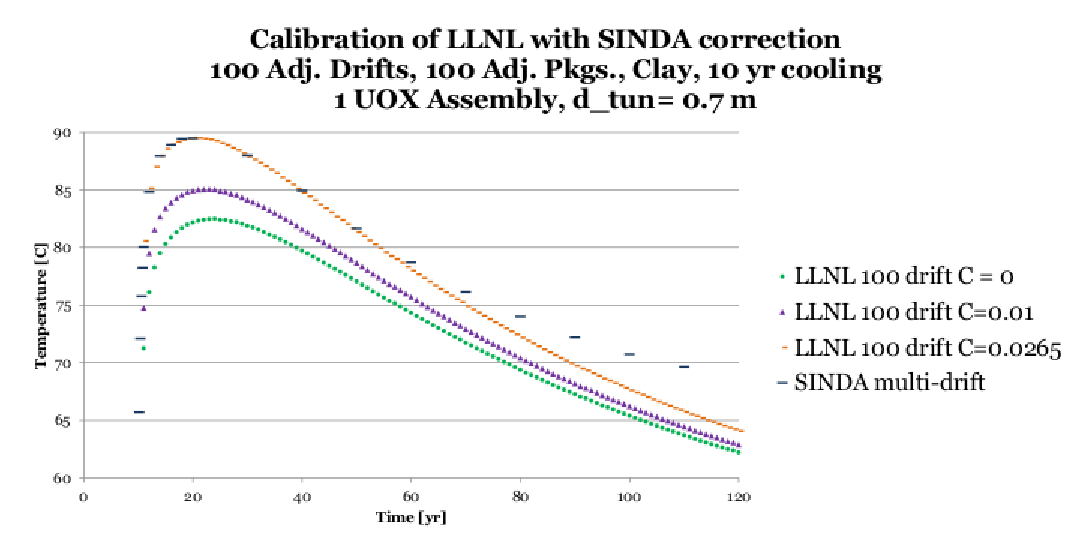
\includegraphics[width=0.5\textwidth]{100drift10yr.eps}
    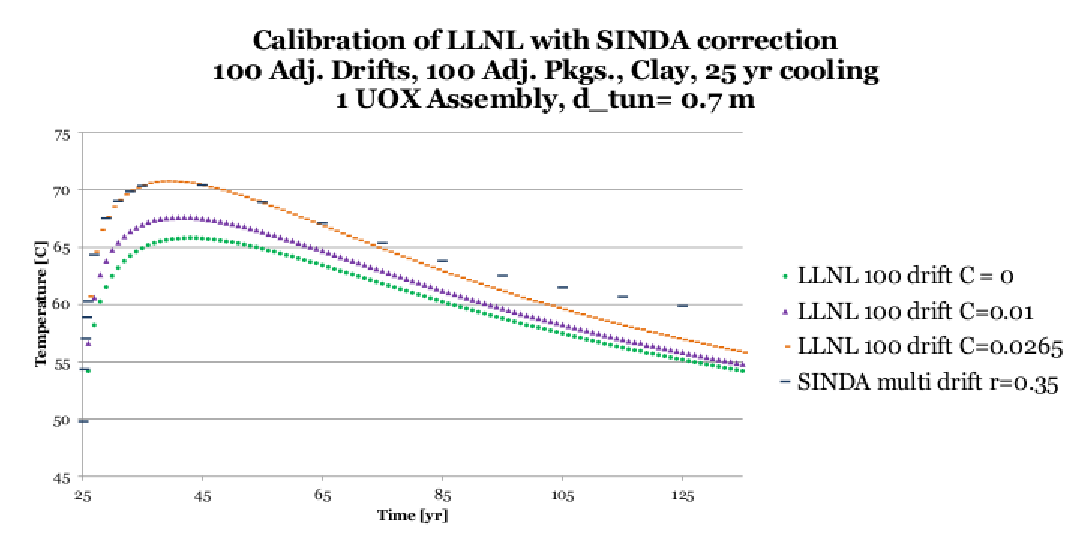
\includegraphics[width=0.5\textwidth]{100drift25yr.eps}
    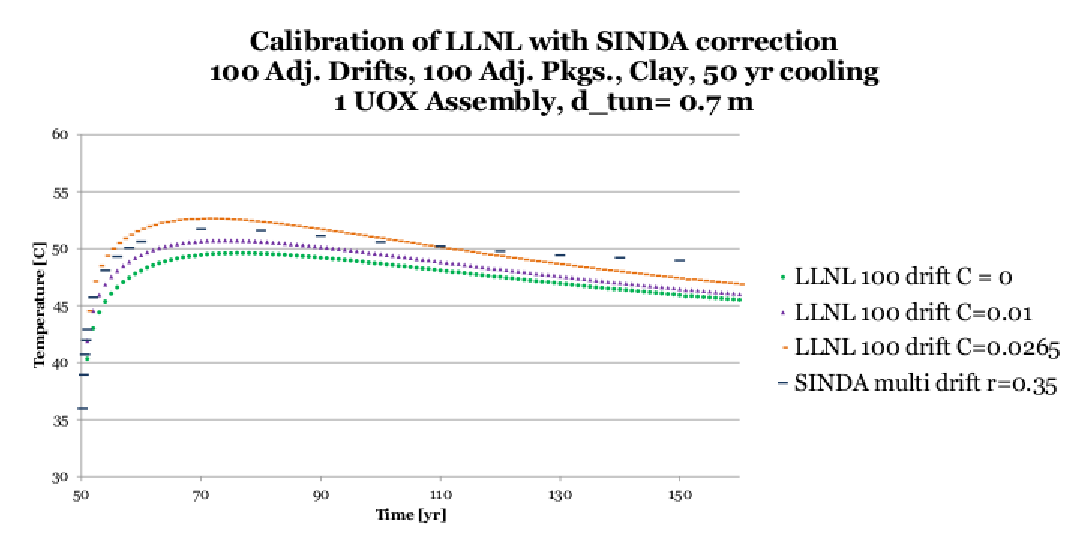
\includegraphics[width=0.5\textwidth]{100drift50yr.eps}
  \caption{Vertical, horizontal, alcove, and borehole emplacement layouts can be 
  represented by a line of point sources and adjacent line sources 
  \cite{sutton_investigations_2011}.}
  \label{fig:llnl}
\end{figure}

\begin{figure}[h!]
  \centering
    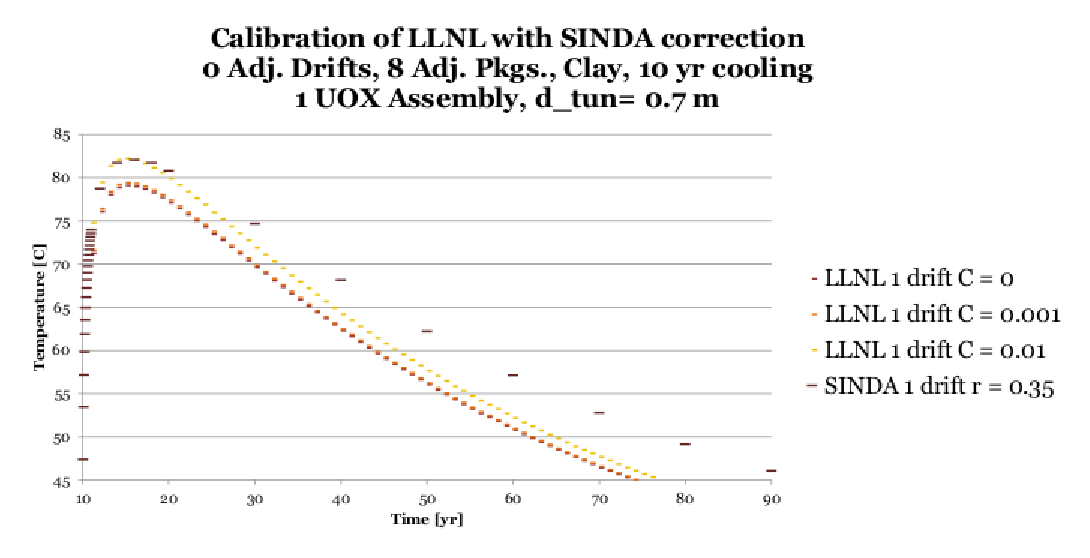
\includegraphics[width=0.5\textwidth]{1drift10yr.eps}
    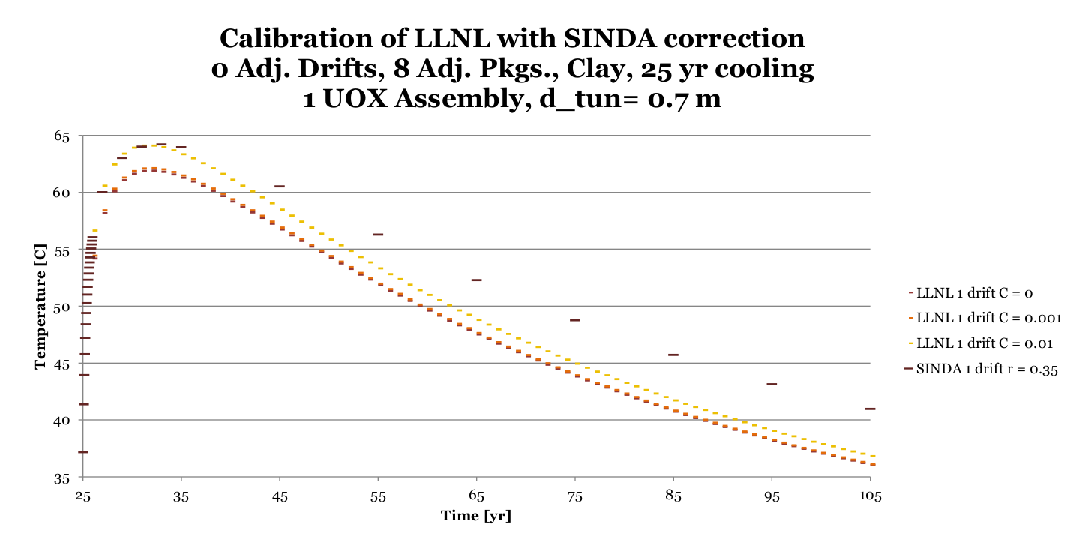
\includegraphics[width=0.5\textwidth]{1drift25yr.eps}
    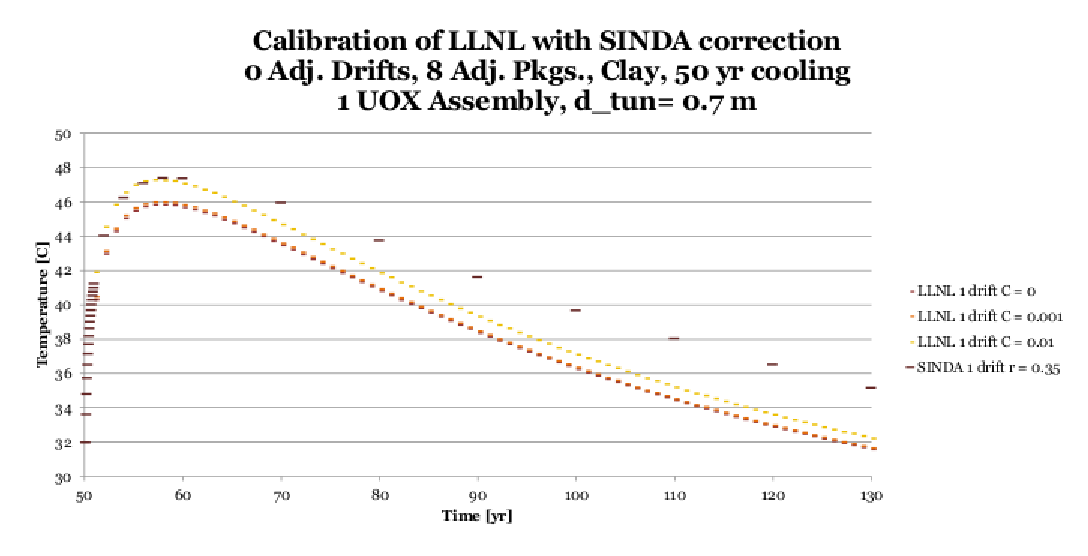
\includegraphics[width=0.5\textwidth]{1drift50yr.eps}
  \caption{Vertical, horizontal, alcove, and borehole emplacement layouts can be 
  represented by a line of point sources and adjacent line sources 
  \cite{sutton_investigations_2011}.}
  \label{fig:llnl}
\end{figure}

% Theory

% Application for Other Analytical Capacity Based models?

The calibration was an improvement on the benchmarking.

%%%%%%%%%%%%%%%%%%%%%%%%%%%%%%%%%%%%%%%%%%%%%%%%%%%%%%%%%%%%%%%%%%%%%%%%%%%%%%%%
\section{Conclusions}

We recommend that for this and other analytical models of this nature, the 
additional step will improve results near the area of interest.

%%%%%%%%%%%%%%%%%%%%%%%%%%%%%%%%%%%%%%%%%%%%%%%%%%%%%%%%%%%%%%%%%%%%%%%%%%%%%%%%
%\nocite{<+ +>}
\bibliographystyle{ans}
\bibliography{ans2012.bib}
\end{document}


